%! TEX root = ../thesis.tex
\section{Deployed System}%
\label{pdk:sec:depsys}

We deploy a Web platform to provide real-time predictions for Swiss referenda\footnote{The platform is available on \href{http://www.predikon.ch}{www.predikon.ch}.}.
Four Sundays a year, Swiss citizens are called on to vote on at least one item in a referendum.
These items can cover a broad range of topics, from joining the European Union to subsidizing railways and roads, from banning the use of fossil fuels to cutting taxes, and even forbidding Swiss farmers to remove horns from cows and goats.
A month prior to a referendum vote day, eligible voters receive official ballots, together with useful documentation.
To cast their vote, they can either send their ballot by post or bring it to the ballot office on the referendum vote day, up to 11:59am.
Starting at 12pm, each municipality is in charge of counting both the remote ballots and the ballots they collected on the same day.
Once they have finished counting, they report the result to their canton whose administration communicates the official count.

\subsection{Implementation Details}

In 2019, the Swiss Federal Statistical Office released a public API to access vote data, both historical and real-time, for all municipalities in a standardized format~\cite{confederation2020open}.
This enabled us to obtain sequential results in all municipalities on the referendum vote days and made it possible to use our algorithm to predict the outcome of referenda starting at 12pm.
We use the dataset described in Table~\ref{pdk:tab:datasets} for Switzerland, which contains~$R = 2196$ municipalities.
We predict the outcome of two items on May 19, 2019, using~$V = 326$ votes and two items on February 9, 2020, using~$V = 328$ votes\footnote{The two referendum vote days between May 19, 2019, and February 9, 2020, were replaced by the Swiss legislative elections in Fall 2019. The referendum vote days after February 9, 2020, were cancelled due to the COVID-19 crisis in Spring 2020.}.
We summarize these four items in Table~\ref{pdk:tab:real_votes}.
The turnout was about 44\% on May 19 and about 42\% on February 9.
For each referendum, about 2.2 million valid ballots were counted.

\begin{table}
	\caption{
		True outcome $y^*_{\textrm{nat}}$, earliest prediction $y_{\textrm{nat}}$, and absolute difference $\Delta = \vert y^*_{\textrm{nat}} - y_{\textrm{nat}} \vert $ for referenda with real data.
	}
	\label{pdk:tab:real_votes}
	\begin{tabular}{llrrr}
		\toprule
		Date   & Item              & $y^*_{\textrm{nat}}$ [\%] & $y_{\textrm{nat}}$ [\%] & $\Delta$ \\
		\midrule

		May 19 & Tax Reform        & 66.38                     & 67.90                   & 1.52     \\
		May 19 & Weapon Regulation & 63.73                     & 63.52                   & 0.21     \\
		Feb 9  & Affordable Houses & 42.95                     & 41.57                   & 1.38     \\
		Feb 9  & Ban on Homophobia & 63.09                     & 62.94                   & 0.15     \\

		\bottomrule
	\end{tabular}
\end{table}

For a vote~$V+1$, we use the historical data up to vote~$V$ to learn the feature matrix~$\vX$ from the sub-matrix~$\vY_V$.
We use a Bernoulli likelihood to define our GLM with~$D=25$ latent dimensions and a regularization factor~$\lambda=0.01$.
We fetch municipal results from the API every two minutes\footnote{Schedule suggested by the Swiss Federal Statistical Office.}.
If new results are available, we learn the optimal parameters~$\vw_*$ by optimizing the negative log-likelihood using Newton's method, and we predict the unobserved municipal results as $\vy_{V+1}^{(\Ubs)} = \sigma(X^{(\Ubs)} \vw_*)$.
We predict the national outcome~$y_{\textrm{nat}} \in [0, 1]$ by aggregating our prediction of unobserved results~$\Ubs$ with the observed results~$\Obs$ as
\begin{equation}
	y_{\textrm{nat}} = \frac{1}{N} \left( \sum_{r \in \Ubs} N_r^{(\Ubs)} y_{r, V+1}^{(\Ubs)} + \sum_{r \in \Obs} N_r^{(\Obs)} y_{r, V+1}^{(\Obs)} \right),
\end{equation}
where~$N_r^{(\Ubs)}$ is the number of valid ballots in municipality~$r$ from the previous vote (used as proxy for the current vote),~$N_r^{(\Obs)}$ is the number of valid ballots in municipality~$r$ for the current vote, and~$N = \sum_{r \in \Ubs} N_r^{(\Ubs)} + \sum_{r \in \Obs} N_r^{(\Obs)}$ is the total number of valid ballots.
As the number of unobserved results~$\vert \Ubs \vert$ tends to 0 with time and the number of observed results~$\vert \Obs \vert$ tends to the total number of regions~$R$, the prediction for the national outcome~$y_{\textrm{nat}}$ converges to the true outcome~$y_{\textrm{nat}}^* \in [0, 1]$.

\subsection{Real-Time Predictions}

In Figure~\ref{pdk:fig:predictions}, we show the evolution of our predictions (solid red line), together with the weighted averaging (solid black line), and the progress of the ballot counting (solid blue line) for the two referenda on February 9, 2020.
The ballot counting starts at 12pm and ends at 4pm, after all municipalities reported their results
Looking at the trajectory of the counting progress, the jumps occurring at several timestamps correspond to the publication of the results of the whole canton of Wallis and the city of Basel at 12:35pm, of Thun at 2:10pm, of Geneva at 2:40pm, and of Bern at 3pm, all of which are major cities in Switzerland.
The large municipality of Zurich is split into nine districts that published their results independently, thus diluting its effect on the counting.

At 12pm, using the results of 531 municipalities (23.9\% of all municipalities) representing 13.2\% of the total population, we predict 41.57\% for the "Affordable Housing" and 62.94\% for the "Ban on Homophobia".
This corresponds to a mean absolute error of 1.38\% and 0.15\% to the true outcome, respectively.
The weighted average for the current count varies up to a difference of 6.5\% and 4.5\%, respectively, whereas our prediction is stable over time.
To provide a robust estimation of the final outcome, our algorithm takes advantage of the correlation across municipalities and votes.
The performance of our approach for the two referenda of May 19, 2019, is similar; but we do not show them\footnote{The interested reader can access these predictions on our \href{http://www.predikon.ch}{Web platform}.}, as early counting data were not available due to a bug on the API side (they published the first results at 12:35pm).
Furthermore, the results of the nine districts of Zurich, which cumulatively form the largest municipality in Switzerland, were incorrectly reported on that day.
Consequently, we could not reliably use the results in our algorithm.
We report only the earliest prediction, made at 12:40pm, in Table~\ref{pdk:tab:real_votes}.

\begin{figure}
	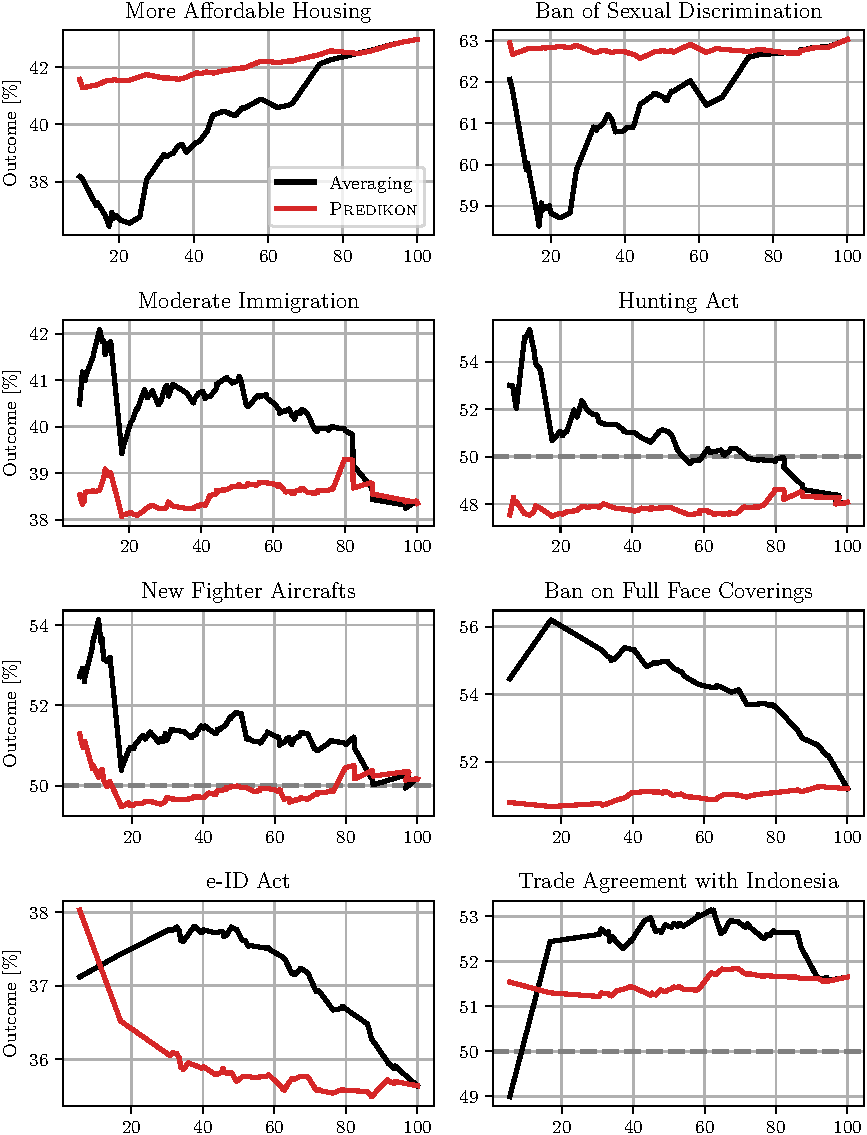
\includegraphics{pdk-predictions.pdf}
	\caption{
		Evolution of predictions (red) and weighted averaging (black) on real, sequential data for the two referenda of February 9, 2020, together with the progress of the ballot counting (blue).
	}
	\label{pdk:fig:predictions}
\end{figure}
